\newpage
\setcounter{section}{3}
\setcounter{subsection}{0}
\Section{Dataset 3: The UCI User Knowledge Modeling}

In this Section, we will present the classification results of the dataset that we used in our project, which is the UCI User Knowledge Modeling dataset \cite{user_knowledge_modeling}.

The User Knowledge Modeling dataset provides real-world data about students' knowledge status on the subject of Electrical DC Machines. The dataset was obtained as part of a Ph.D. thesis and has been analyzed to classify the knowledge levels of students based on various input features. The knowledge classes were determined in the thesis using a hybrid machine learning technique combining k-Nearest Neighbors (k-NN) with meta-heuristic exploration methods.

\subsubsection*{Dataset Characteristics}
\begin{itemize}
    \item \textbf{Type:} Multivariate
    \item \textbf{Subject Area:} Computer Science
    \item \textbf{Associated Tasks:} Classification, Clustering
    \item \textbf{Feature Type:} Integer
    \item \textbf{Number of Instances:} 403
    \item \textbf{Number of Features:} 5
    \item \textbf{Missing Values:} No
\end{itemize}

\subsubsection*{Dataset Insights}
\begin{itemize}
    \item \textbf{Objective:} To classify students' knowledge levels about Electrical DC Machines into predefined classes based on input features related to study habits and exam performance.
    \item \textbf{Classification Methodology:} The authors utilized an intuitive knowledge classifier, which combines k-Nearest Neighbor (k-NN) with meta-heuristic methods for classifying knowledge levels.
    \item \textbf{Class Distribution:} The dataset contains imbalanced classes:
    \begin{itemize}
        \item Very Low: 50 instances
        \item Low: 129 instances
        \item Middle: 122 instances
        \item High: 102 instances
    \end{itemize}
\end{itemize}

\subsubsection*{Feature Description}
\begin{itemize}
    \item \textbf{Input Variables:}
    \begin{enumerate}
        \item \textbf{STG:} The degree of study time for goal object materials.
        \item \textbf{SCG:} The degree of repetition of goal object materials.
        \item \textbf{STR:} The degree of study time for related objects with the goal object.
        \item \textbf{LPR:} The exam performance for related objects with the goal object.
        \item \textbf{PEG:} The exam performance for the goal objects.
    \end{enumerate}
    \item \textbf{Output Variable:}
    \begin{itemize}
        \item \textbf{UNS:} The knowledge level of the user, classified into four categories:
        \begin{enumerate}
            \item Very Low
            \item Low
            \item Middle
            \item High
        \end{enumerate}
    \end{itemize}
\end{itemize}

\subsection{Data preparation}

\subsubsection{Import the dataset}

The \href{https://archive.ics.uci.edu/}{UC Irvine Machine Learning Repository} allows for direct dataset import in Python using the \texttt{ucimlrepo} package. The package is included in the \texttt{requirements.txt} file. The following code demonstrates how to import the Wine Quality (id = 257) dataset using the \texttt{fetch\_ucirepo} function:

\lstset{style=code}
\begin{lstlisting}[language=Python]
from ucimlrepo import fetch_ucirepo 

breast_cancer_wisconsin_diagnostic = fetch_ucirepo(id=257) 
    
X = breast_cancer_wisconsin_diagnostic.data.features 
y = breast_cancer_wisconsin_diagnostic.data.targets 
\end{lstlisting}

\subsubsection{Splitting the dataset}

The dataset is split into training and testing sets using the \texttt{train\_test\_split} function from the \texttt{sklearn} library. 
The dataset is splitted into 4 sets of different test sizes: 60\%, 40\%, 20\%, and 10\% of the dataset in stratified fashion, using the random state of 22125 to ensure reproducibility.

\begin{figure}[H]
    \centering
    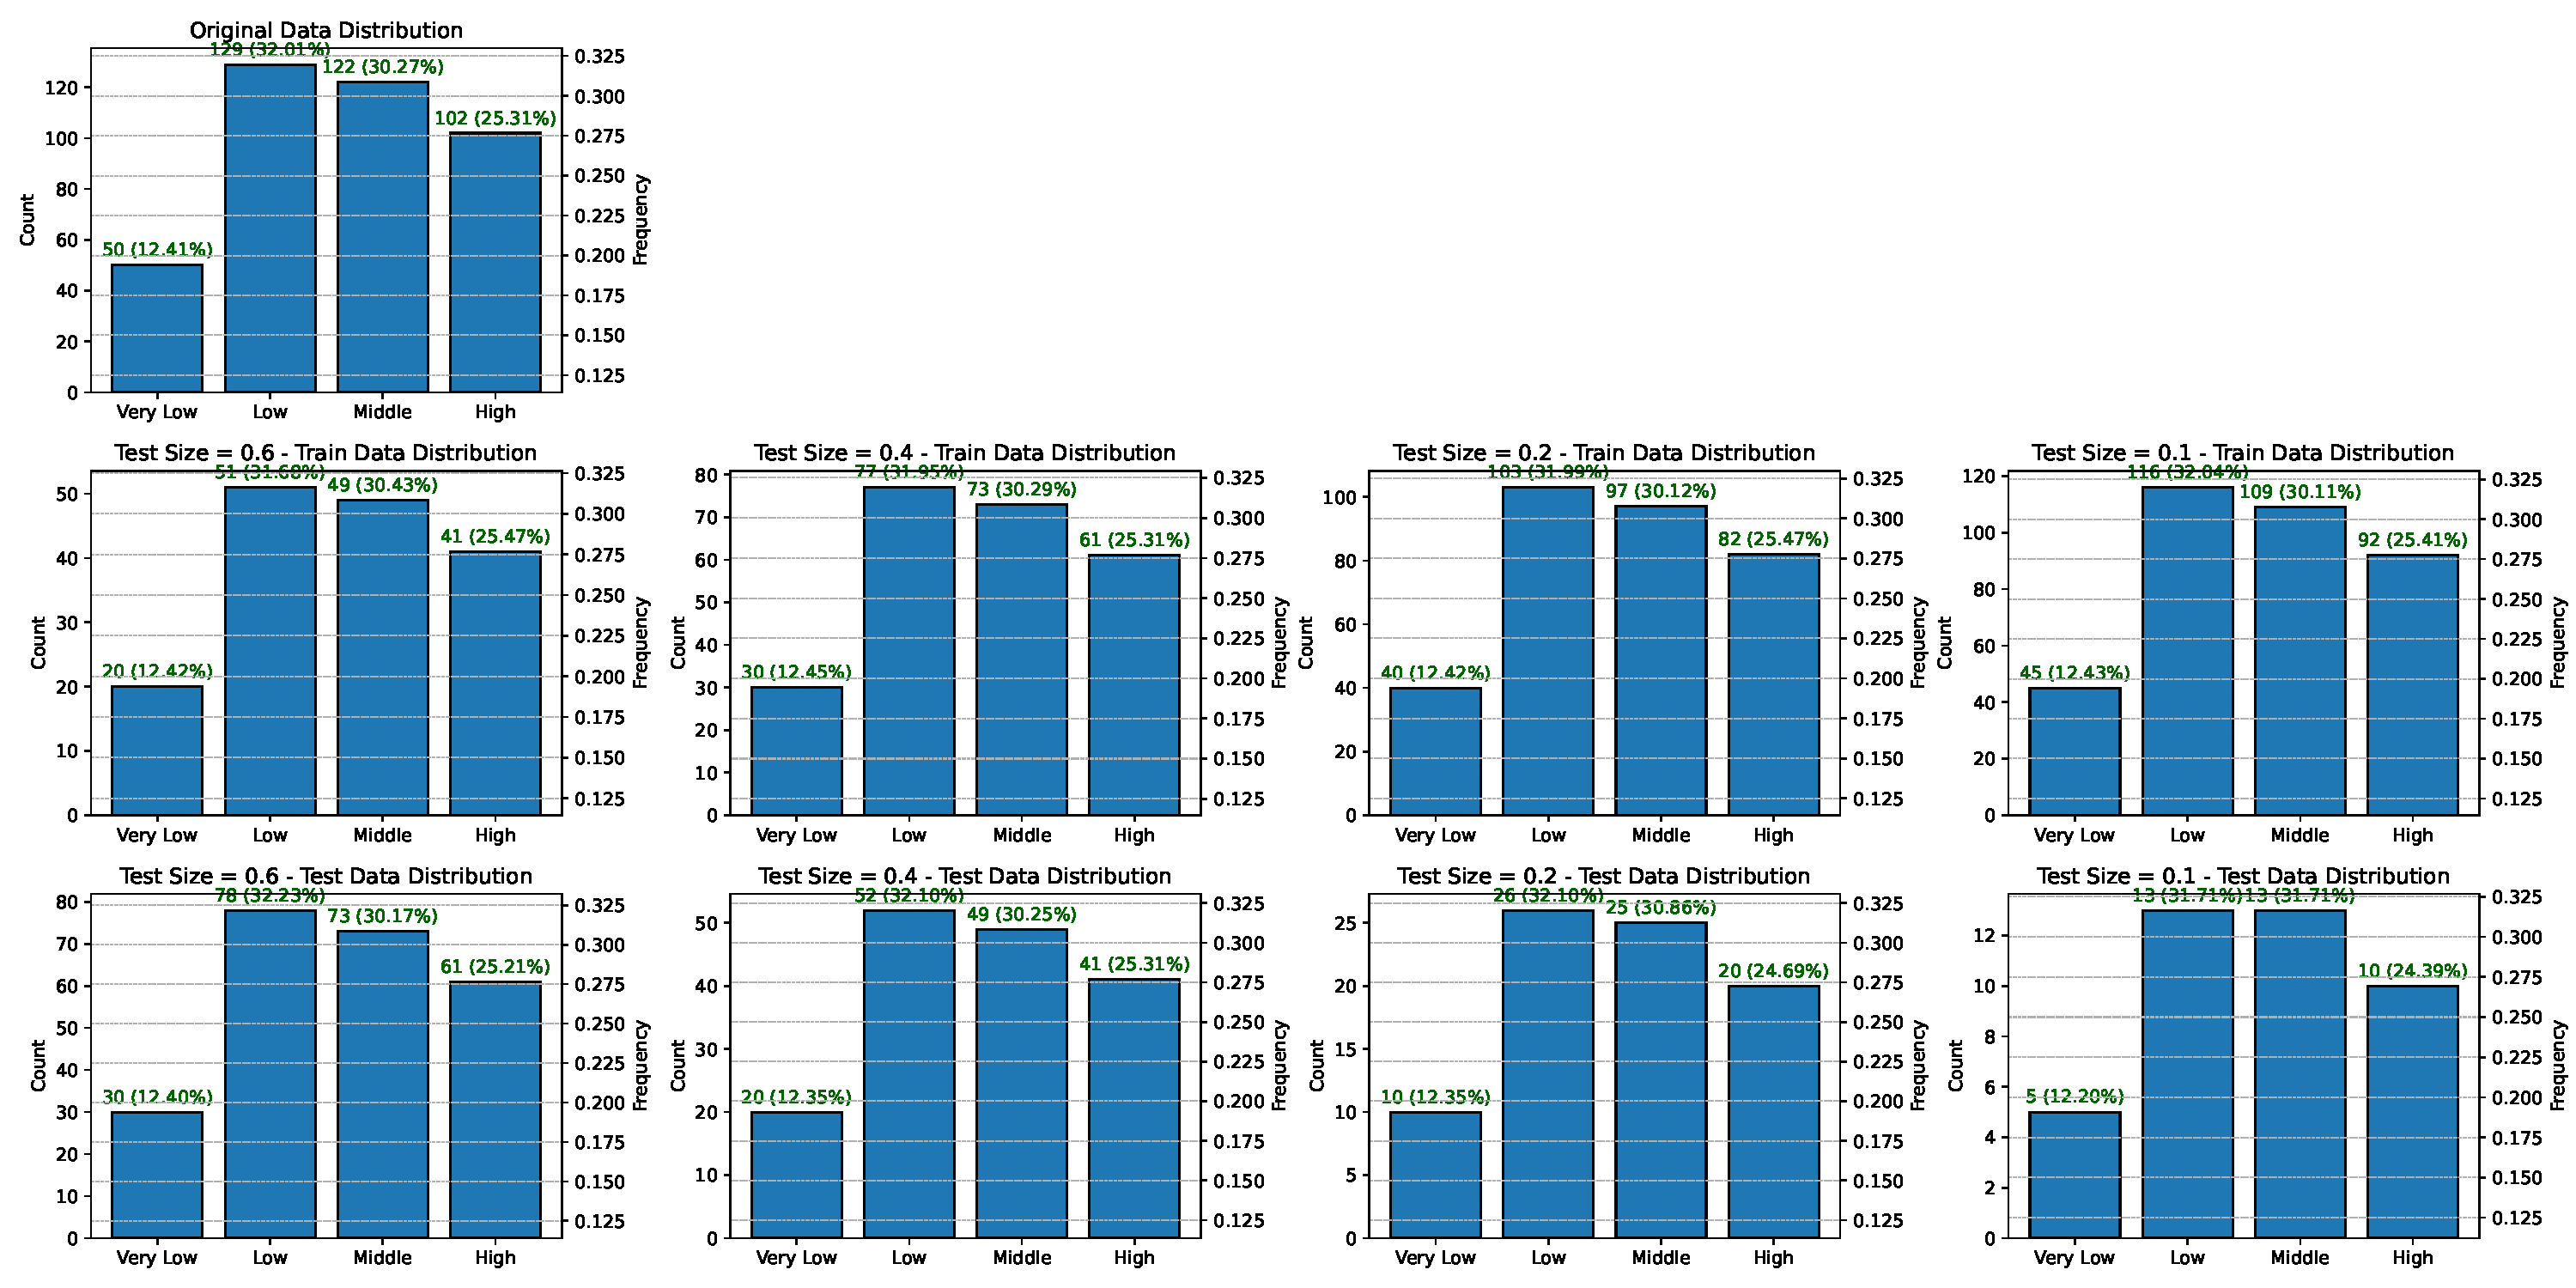
\includegraphics[width=\textwidth]{figures/user_knowledge_modeling_split.pdf}
    \caption{User Knowledge Modeling dataset splits}
    \label{fig:user_knowledge_modeling_split}
\end{figure}

As shown in figure \ref{fig:user_knowledge_modeling_split}, the distribution of the target class is preserved in all splits.

\subsection{Decision Tree classifier implementation}

Decision Tree classifiers are implemented using the \texttt{DecisionTreeClassifier} class from the \texttt{sklearn} library. 
To ensure reproducibility, the random state is set to 22125. 
We use the Entropy (information gain) criterion to split the nodes and set the maximum depth of the tree to None to allow the tree to grow until all leaves are pure.

\begin{figure}[H]
    \centering
    \includegraphics[width=\textwidth]{figures/user_knowledge_modeling_decision_trees.pdf}
    \caption{User Knowledge Modeling dataset Decision Trees with different test sizes}
    \label{fig:user_knowledge_modeling_decision_trees}
\end{figure}

The Decision Trees are visualized in figure \ref{fig:user_knowledge_modeling_decision_trees}. The trees grow deeper as the test size decreases, indicating that the model is more complex and overfits the training data when the test size is small.

The first node of the Decision Tree agrees on the feature \texttt{PEG} to split the dataset for all test sizes. This feature is likely the most discriminative for classifying the knowledge levels of students.

The first node's entropy is approximately 1.924 in all Decision Trees, indicating that the first split is not very informative. However, the Decision Tree classifier effectively splits the dataset into pure leaves with high information gain.

\subsection{Performance evaluation}

\subsubsection{Classification report}

The classification report provides a comprehensive evaluation of the Decision Tree classifier's performance using the \texttt{classification\_report} function from the \texttt{sklearn.metrics} module. The report includes the following metrics:
\begin{itemize}
    \item \textbf{Precision:} The ratio of true positive samples to the sum of true positive and false positive samples.
    \item \textbf{Recall:} The ratio of true positive samples to the sum of true positive and false negative samples.
    \item \textbf{F1-score:} The harmonic mean of precision and recall.
    \item \textbf{Support:} The number of samples in each class.
\end{itemize}

\textbf{Classification Report for Test Size = 0.6}

\begin{tabular}{lcccccc}
\hline
 & \textbf{Precision} & \textbf{Recall} & \textbf{F1-score} & \textbf{Support} \\
\hline
Very Low & 0.89 & 0.80 & 0.84 & 30 \\
Low & 0.87 & 0.88 & 0.88 & 78 \\
Middle & 0.88 & 0.84 & 0.86 & 73 \\
High & 0.88 & 0.97 & 0.92 & 61 \\
\hline
\textbf{Accuracy} & & & 0.88 & 242 \\
\textbf{Macro avg} & 0.88 & 0.87 & 0.88 & 242 \\
\textbf{Weighted avg} & 0.88 & 0.88 & 0.88 & 242 \\
\hline
\end{tabular}

\vspace{2em}

\textbf{Classification Report for Test Size = 0.4}

\begin{tabular}{lcccccc}
\hline
 & \textbf{Precision} & \textbf{Recall} & \textbf{F1-score} & \textbf{Support} \\
\hline
Very Low & 0.84 & 0.80 & 0.82 & 20 \\
Low & 0.88 & 0.88 & 0.88 & 52 \\
Middle & 0.94 & 0.92 & 0.93 & 49 \\
High & 0.95 & 1.00 & 0.98 & 41 \\
\hline
\textbf{Accuracy} & & & 0.91 & 162 \\
\textbf{Macro avg} & 0.90 & 0.90 & 0.90 & 162 \\
\textbf{Weighted avg} & 0.91 & 0.91 & 0.91 & 162 \\
\hline
\end{tabular}

\vspace{2em}

\textbf{Classification Report for Test Size = 0.2}

\begin{tabular}{lcccccc}
\hline
 & \textbf{Precision} & \textbf{Recall} & \textbf{F1-score} & \textbf{Support} \\
\hline
Very Low & 1.00 & 0.70 & 0.82 & 10 \\
Low & 0.81 & 1.00 & 0.90 & 26 \\
Middle & 1.00 & 0.80 & 0.89 & 25 \\
High & 0.91 & 1.00 & 0.95 & 20 \\
\hline
\textbf{Accuracy} & & & 0.90 & 81 \\
\textbf{Macro avg} & 0.89 & 0.88 & 0.93 & 81 \\
\textbf{Weighted avg} & 0.90 & 0.90 & 0.92 & 81 \\
\hline
\end{tabular}

\vspace{200em}

\textbf{Classification Report for Test Size = 0.1}

\begin{tabular}{lcccccc}
\hline
 & \textbf{Precision} & \textbf{Recall} & \textbf{F1-score} & \textbf{Support} \\
\hline
Very Low & 1.00 & 0.40 & 0.57 & 5 \\
Low & 0.68 & 1.00 & 0.81 & 13 \\
Middle & 1.00 & 0.62 & 0.76 & 13 \\
High & 0.83 & 1.00 & 0.91 & 10 \\
\hline
\textbf{Accuracy} & & & 0.80 & 41 \\
\textbf{Macro avg} & 0.76 & 0.75 & 0.88 & 41 \\
\textbf{Weighted avg} & 0.79 & 0.80 & 0.86 & 41 \\
\hline
\end{tabular}

The classification reports show that the Decision Tree classifier achieves high precision, recall, and F1-score for all classes in the test data. The model has an accuracy of approximately 0.88, 0.91, 0.90, and 0.80 for test sizes of 60\%, 40\%, 20\%, and 10\%, respectively. The model performs well in classifying the knowledge levels of students based on the input features.

\subsubsection{Confusion matrix}

The confusion matrix provides a visual representation of the Decision Tree classifier's performance using the \texttt{confusion\_matrix} function from the \texttt{sklearn.metrics} module. The matrix shows the number of true positive, false positive, true negative, and false negative samples for each class.

\begin{figure}[H]
    \centering
    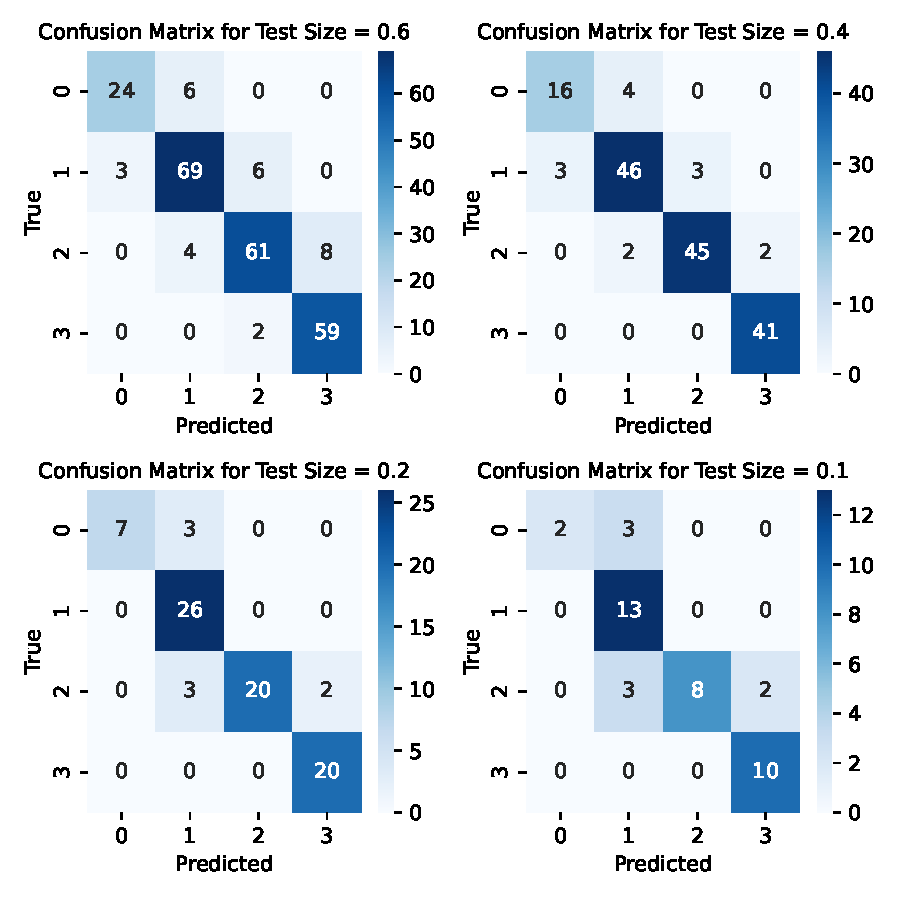
\includegraphics[width=.7\textwidth]{figures/user_knowledge_modeling_confusion_matrices.pdf}
    \caption{User Knowledge Modeling dataset Confusion Matrices with different test sizes}
    \label{fig:user_knowledge_modeling_confusion_matrices}
\end{figure}
% Confusion Matrix for Test Size = 0.6:
% [[24  6  0  0]
%  [ 3 69  6  0]
%  [ 0  4 61  8]
%  [ 0  0  2 59]]
% Confusion Matrix for Test Size = 0.4:
% [[16  4  0  0]
%  [ 3 46  3  0]
%  [ 0  2 45  2]
%  [ 0  0  0 41]]
% Confusion Matrix for Test Size = 0.2:
% [[ 7  3  0  0]
%  [ 0 26  0  0]
%  [ 0  3 20  2]
%  [ 0  0  0 20]]
% Confusion Matrix for Test Size = 0.1:
% [[ 2  3  0  0]
%  [ 0 13  0  0]
%  [ 0  3  8  2]
%  [ 0  0  0 10]]

The confusion matrices in figure \ref{fig:user_knowledge_modeling_confusion_matrices} show that the Decision Tree classifier correctly classifies most samples in the test data. The classifier has high true positive rates for all classes, indicating that the model effectively identifies the knowledge levels of students.

\subsection{Depth vs Accuracy evaluation}

The Decision Tree classifier's performance is evaluated by varying the maximum depth of the tree. The accuracy of the classifier is computed for different maximum depths using the \texttt{accuracy\_score} function from the \texttt{sklearn.metrics} module for the Decision Tree classifier with a test size of 20\%.

\begin{figure}[H]
    \centering
    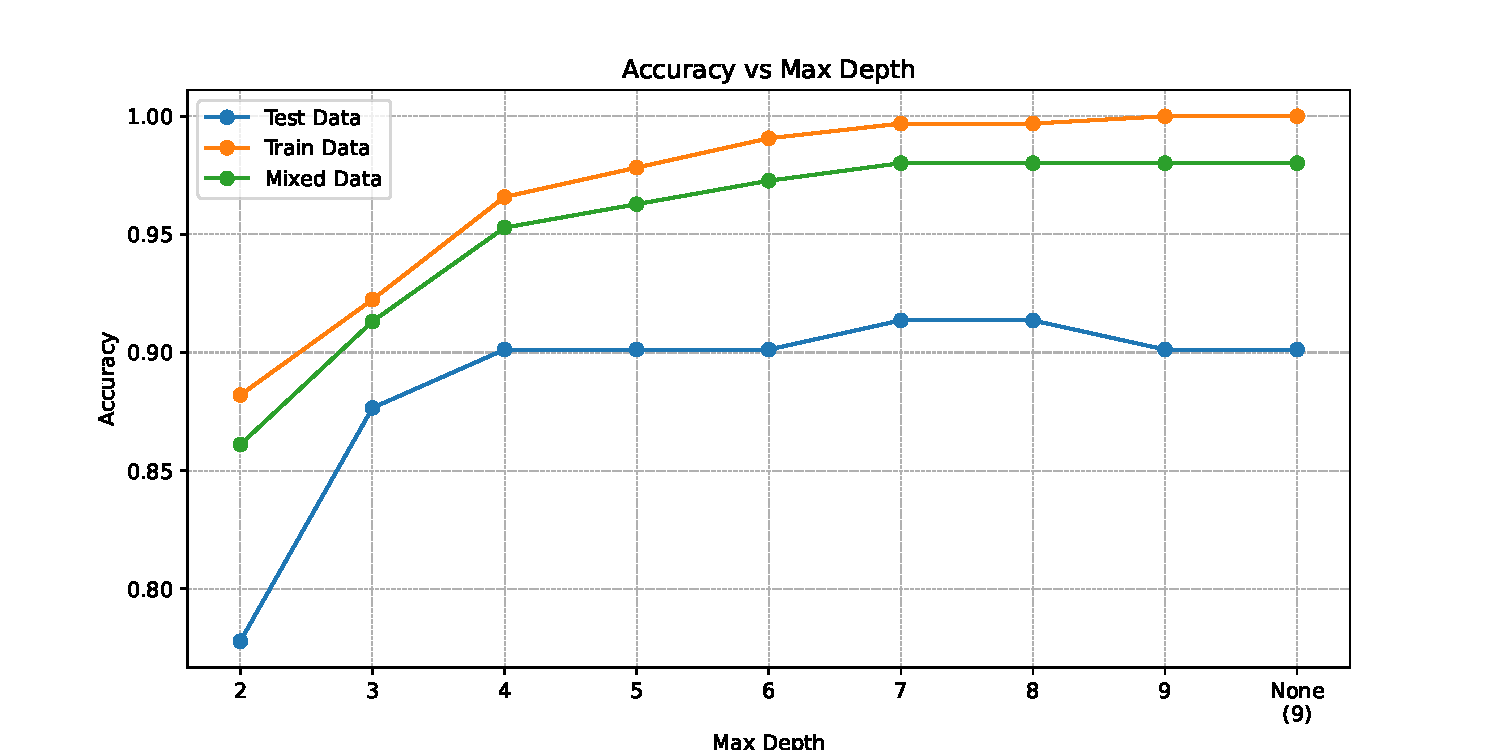
\includegraphics[width=\textwidth]{figures/user_knowledge_modeling_accuracy_vs_max_depth.pdf}
    \caption{User Knowledge Modeling dataset Depth vs Accuracy}
    \label{fig:user_knowledge_modeling_accuracy_vs_max_depth}
\end{figure}

The plot in figure \ref{fig:user_knowledge_modeling_accuracy_vs_max_depth} shows that the Decision Tree classifier achieves the highest accuracy on the test data when the maximum depth is around 7. The accuracy decreases slightly as the maximum depth increases beyond 7, indicating that the model starts to overfit the training data but still performs well on the test data.

